\documentclass[11pt,a4paper]{report}

%% =============================================================
%%  main.tex
%%  Sensor Fusion of Camera and Pressure Sensor Data for Cabin
%%  Monitoring System
%%  Master Thesis -- Deggendorf Institute of Technology, Campus Cham
%% =============================================================

%% =============================================================
%%  preamble.tex
%%  Package configuration for the Campus Cham Master Thesis template
%% =============================================================

%% ---------------- Encoding, language, fonts -----------------------
\usepackage[T1]{fontenc}
\usepackage[utf8]{inputenc}
\usepackage[english]{babel}

%% Helvetica/Arial-equivalent sans-serif font, as required by the
%% Campus Cham thesis guideline.
\usepackage{helvet}
\renewcommand{\familydefault}{\sfdefault}

%% ---------------- Page geometry -----------------------------------
\usepackage[a4paper,top=2.5cm,bottom=2.5cm,left=3cm,right=2cm]{geometry}

%% ---------------- Line spacing (1.5) -------------------------------
\usepackage{setspace}
\onehalfspacing

%% ---------------- Micro-typography ---------------------------------
\usepackage{microtype}

%% ---------------- Headings: chapter / section / subsection sizes ----
\usepackage{titlesec}

%% Chapter heading: 14pt bold, no "Chapter X" prefix -- shows "1 Introduction"
\titleformat{\chapter}[hang]
  {\normalfont\fontsize{14pt}{16pt}\selectfont\bfseries}
  {\thechapter}
  {1em}
  {}
\titlespacing*{\chapter}{0pt}{0pt}{20pt}

%% Section heading: 12pt bold
\titleformat{\section}
  {\normalfont\fontsize{12pt}{14pt}\selectfont\bfseries}
  {\thesection}
  {1em}
  {}

%% Subsection heading: 11pt bold
\titleformat{\subsection}
  {\normalfont\fontsize{11pt}{13pt}\selectfont\bfseries}
  {\thesubsection}
  {1em}
  {}

%% Numbering depth: 1, 1.1, 1.1.1 (max 3 levels)
\setcounter{secnumdepth}{3}
\setcounter{tocdepth}{3}

%% ---------------- Header / footer -----------------------------------
\usepackage{fancyhdr}
\pagestyle{fancy}
\fancyhf{} % clear all header/footer fields
\fancyfoot[R]{\thepage} % page number, right-aligned, footer only
\renewcommand{\headrulewidth}{0pt} % no header rule -- no header content
\fancypagestyle{plain}{%
  \fancyhf{}
  \fancyfoot[R]{\thepage}
  \renewcommand{\headrulewidth}{0pt}
}

%% ---------------- Graphics, captions, tables -------------------------
\usepackage{graphicx}
\usepackage{caption}
\captionsetup{font=small,labelfont=bf}
\usepackage{subcaption}
\usepackage{booktabs}
\usepackage{float}
\usepackage{longtable}

%% ---------------- Maths -----------------------------------------------
\usepackage{amsmath}
\usepackage{amssymb}

%% ---------------- Colour -----------------------------------------------
\usepackage{xcolor}

%% ---------------- Hyperlinks and cross-references -----------------------
\usepackage{hyperref}
\hypersetup{
  colorlinks=false,
  pdfborder={0 0 0},
  pdftitle={Sensor Fusion of Camera and Pressure Sensor Data for Cabin Monitoring System},
  pdfauthor={CHETHAN SRINIVASAREDDY}
}
\usepackage{cleveref}

%% ---------------- Bibliography (numeric, order of citation) -------------
\usepackage[backend=bibtex,style=numeric,sorting=none,citestyle=numeric-comp]{biblatex}
\addbibresource{bibliography.bib}

%% ---------------- Draft annotations --------------------------------------
%% GUIDANCE: Set disable=true before final submission to hide all \todo notes.
\usepackage[colorinlistoftodos,textsize=footnotesize,disable=false]{todonotes}

%% =============================================================
%% NOTE ON ABBREVIATIONS LIST
%% The glossaries package is intentionally NOT used here because its
%% \makeglossaries / makeindex-based build step conflicts with the
%% biblatex + bibtex workflow requested for this project. The List of
%% Abbreviations is instead built manually as a two-column longtable in
%% chapters/00_frontmatter.tex.
%% =============================================================


\graphicspath{{figures/}}

\begin{document}

%% =============================================================
%% FRONT MATTER (roman page numbers)
%% =============================================================
\pagenumbering{roman}
\setcounter{page}{1}

%% ---------------- Title Page ----------------------------------
\begin{titlepage}
\centering

{\large Deggendorf Institute of Technology\par}
{\large Campus Cham\par}
\vspace{0.3cm}
{\large Course Name\par}

\vspace{1.5cm}

%% GUIDANCE: Replace the rule below with \includegraphics{figures/dit_logo}
%% once the official DIT / Campus Cham logo file is available.
\fbox{\parbox[c][3cm][c]{6cm}{\centering \todo[inline]{Insert DIT / Campus Cham logo here (figures/dit\_logo.pdf)}}}

\vspace{2cm}

{\Large \textbf{MASTER THESIS}\par}

\vspace{1.5cm}

{\Large \textbf{Sensor Fusion of Camera and Pressure Sensor Data\\ for Cabin Monitoring System}\par}

\vspace{1.5cm}

{\large submitted in the requirements for the degree of\par}
\vspace{0.2cm}
{\large \textbf{Master of Engineering}\par}

\vspace{2cm}

{\large by\par}
\vspace{0.2cm}
{\large \textbf{CHETHAN SRINIVASAREDDY}\par}
\vspace{0.2cm}
{\large Matriculation Number: \todo{Insert matriculation number}\par}

\vspace{1.5cm}

{\large Supervisor: [SUPERVISOR NAME]\par}
%% TODO: Add second supervisor / external examiner line if required by Campus Cham guideline.

\vspace{1.5cm}

{\large Cham, 2026\par}

\end{titlepage}

%% ---------------- Restriction Note (disabled by default) ------
%% GUIDANCE: If this thesis contains confidential company data, remove
%% the \iffalse / \fi wrapper below to activate the restriction note,
%% and fill in the company name and restriction period.
\iffalse
\thispagestyle{empty}
\vspace*{4cm}
\begin{center}
\textbf{Restriction Note}
\end{center}
\noindent This thesis contains confidential information of \todo{Company Name}.
It may only be made available to the first and second examiners and
authorised members of the examination board. Publication and duplication
of this thesis, even in part, is prohibited for a period of \todo{X years}
from the date of submission without the express permission of
\todo{Company Name}.
\newpage
\fi

%% ---------------- Acknowledgements ------------------------------
\chapter*{Acknowledgements}
\addcontentsline{toc}{chapter}{Acknowledgements}
I would like to express my sincere gratitude to my supervisor, [SUPERVISOR NAME],
for the continuous guidance, constructive feedback, and support provided
throughout the course of this thesis. I would further like to thank the
research group at Deggendorf Institute of Technology, Campus Cham, for
providing access to the laboratory infrastructure used for pressure sensor
and camera data collection. Finally, I am grateful to my family and friends
for their patience and encouragement during this work.
%% TODO: Personalise acknowledgements with actual names of supervisors,
%% colleagues, funding bodies, or companies that supported this thesis.
\newpage

%% ---------------- Statement of Authorship ------------------------
\chapter*{Statement of Authorship}
\addcontentsline{toc}{chapter}{Statement of Authorship}
I hereby declare that I have authored this thesis independently, that I
have not used other than the declared sources and aids, and that I have
explicitly marked all material which has been quoted either literally or
by content from the sources used. This thesis has not been submitted,
either in part or as a whole, for any other academic degree or examination
at this or any other institution. I am aware that any false statement
regarding this declaration may lead to the invalidation of this thesis
and may have legal consequences.

\vspace{2cm}

\noindent Cham, 2026 \hfill \makebox[6cm]{\hrulefill}

\noindent \hfill [CHETHAN SRINIVASAREDDY]
\newpage

%% ---------------- Abstract ---------------------------------------
\chapter*{Abstract}
\addcontentsline{toc}{chapter}{Abstract}
In-cabin occupant monitoring is increasingly required by vehicle safety
regulation and by advanced restraint systems that must adapt to who is
seated where. This thesis investigates the fusion of RGB camera images
with pressure heatmaps obtained from seat-embedded pressure sensors in
order to jointly estimate seat occupancy, passenger class, occupant
weight, and body pose. A synthetic pressure heatmap generation pipeline
based on human body simulation is proposed to complement limited real
sensor data, together with a Sim2Real validation procedure that quantifies
the remaining domain gap. A multi-task deep learning fusion architecture
combining camera and pressure branches is designed, trained, and evaluated
against single-modality baselines through ablation studies. The expected
contribution is a validated fusion pipeline and dataset methodology that
improves robustness of occupant state estimation over either sensing
modality used in isolation.

\vspace{0.5cm}
\noindent \textbf{Keywords:} cabin monitoring, sensor fusion, pressure heatmap, occupant classification, pose estimation, Sim2Real, multi-task learning
%% TODO: Replace with final abstract (approx. 250-300 words) once results are finalised.
\newpage

%% ---------------- Table of Contents / Figures / Tables ------------
\tableofcontents
\newpage
\listoffigures
\newpage
\listoftables
\newpage

%% ---------------- List of Abbreviations ----------------------------
%% =============================================================
%%  chapters/00_frontmatter.tex
%%  List of Abbreviations (manual longtable).
%%  Title page, acknowledgements, statement of authorship and
%%  abstract are placed directly in main.tex; this file is
%%  \input at the point where the List of Abbreviations should
%%  appear (after List of Tables, before the main matter).
%% =============================================================

\chapter*{List of Abbreviations}
\addcontentsline{toc}{chapter}{List of Abbreviations}

\begin{longtable}{@{}p{3.5cm}p{10cm}@{}}
\toprule
\textbf{Abbreviation} & \textbf{Meaning} \\
\midrule
\endhead
CNN      & Convolutional Neural Network \\
DMS      & Driver Monitoring System \\
EKF      & Extended Kalman Filter \\
FOV      & Field of View \\
GDPR     & General Data Protection Regulation \\
IMU      & Inertial Measurement Unit \\
IR       & Infrared \\
MSE      & Mean Squared Error \\
OMS      & Occupant Monitoring System \\
RGB-D    & Red-Green-Blue plus Depth (image with depth channel) \\
ROI      & Region of Interest \\
Sim2Real & Simulation-to-Reality (transfer) \\
ToF      & Time-of-Flight \\
UKF      & Unscented Kalman Filter \\
WRMSE    & Weighted Root Mean Squared Error \\
\bottomrule
\end{longtable}

%% TODO: Add any further abbreviations introduced in later chapters
%% (e.g. model or dataset acronyms) and keep this list alphabetically sorted.


%% =============================================================
%% MAIN MATTER (arabic page numbers)
%% =============================================================
\cleardoublepage
\pagenumbering{arabic}
\setcounter{page}{1}

%% =============================================================
%%  chapters/01_introduction.tex
%% =============================================================
\chapter{Introduction}
\label{ch:introduction}
%% 1-2 pages of content, including references to relevant literature, that explain

\section{Motivation and Relevance}
\label{sec:motivation}
Occupant monitoring is becoming an increasingly important component of modern vehicle safety systems.
Traditionally, vehicle restraint systems were designed around relatively constrained assumptions:
occupants were expected to be seated in approximately upright, forward-facing positions, and 
the driver was expected to remain continuously engaged in the driving task
\cite{mcmurry2018crash}.
These assumptions are becoming less representative as vehicles incorporate higher levels of driving automation, 
more configurable interiors, and a wider range of in-cabin activities. 
In highly automated vehicles, occupants may increasingly recline, rotate their seats, interact with other passengers,
use mobile devices, work, or perform other non-driving-related activities
\cite{mcmurry2018crash}. Consequently,
the vehicle must account not only for whether a seat is occupied, 
but also \emph{who or what occupies the seat and how the occupant is positioned}.




%% why it is important to fuse camera and pressure data, and how it can improve occupant monitoring performance.
%% what are the limitations of single-modality systems.
%% TODO: Expand with concrete regulatory drivers (e.g. Euro NCAP roadmap,
%% GTR requirements) and cite recent OEM occupant monitoring deployments.


\section{Problem Statement}
\label{sec:problem-statement}
Existing occupant classification systems typically rely on a single
sensing modality, which limits their robustness across the wide range of
seating configurations, occupant sizes, and environmental conditions
encountered in real vehicles. Furthermore, collecting sufficiently large
and diverse real-world pressure sensor datasets is costly and raises data
protection concerns, motivating the use of synthetic data generation.
This thesis addresses the problem of designing, training, and evaluating
a multi-task fusion model that jointly estimates occupancy, passenger
class, weight, and pose from synchronised camera and pressure heatmap
inputs.
\cite{sviro} \cite{ticam} \cite{driveandact} \cite{dmd}


%% TODO: Showing the limitations of single-modality systems and the proposed multi-modal fusion approach aim to solve. 
%% 1.Modality imbalance in the literature: published in-cabin datasets and methods are overwhelmingly vision-based, 
%% need for backup due to its limitations (occlusion, lighting, privacy).

%% By iterating EURO NCAP requirements and how the proposed system can help to meet them, 
%% the problem statement can be strengthened.


\section{Research Questions}
\label{sec:research-questions}
The following research questions guide the design, implementation, and
evaluation carried out in this thesis:
" evaluvating suitability of heterogeneous fusion framework for the proposed modalities,comapring its peformance
 to single-modality baselines".

\begin{enumerate}
    \item Fusion Benefits: To what extent does fusing camera and pressure heatmap data
    improve occupancy, passenger classification, weight estimation, and
    pose estimation accuracy compared to single-modality baselines?
    \item Suitability of fusion architecture for these modalities? 
    \item How should synthetic pressure heatmaps be generated and
    validated to ensure they are statistically representative of real
    seat pressure sensor recordings (Sim2Real gap)? \cite{clever2020bodiesrest3dhuman}
    \item Which feature-level fusion strategy provides the best trade-off
    between accuracy and computational cost for a real-time cabin
    monitoring application?
    \item degradation and abstention : how well can it peform under occlusion, lighting changes, faulty pressure sensor data and other adverse conditions, and
     can it abstain from making predictions when one of the modalities is uncertain/low quality input?
\end{enumerate}

\cite{mobihoc} this is a novel deep fusion architecture that can be used to answer the above research questions.


%% TODO: Confirm the final wording of the research questions with the, remove above references.
%% supervisor and ensure they are consistently revisited in Chapter 9.

\section{Objectives and Scope}
\label{sec:objectives-scope}
The primary objective of this thesis is to design and evaluate a
multi-task deep learning architecture that fuses camera images and
pressure heatmaps for cabin occupant state estimation. The scope covers
system requirements definition, data collection , synthetic  pressure heatmaps generation 
generation via human body simulation, a preprocessing and synchronisation
pipeline, the fusion architecture itself, and a quantitative evaluation
including ablation studies.

%% TODO: Add a bullet-point delimitation list of in-scope vs. out-of-scope
%% items once the experimental setup is finalised.

\section{Thesis Structure}
\label{sec:thesis-structure}
Chapter~\ref{ch:background} introduces the background and fundamentals of
cabin monitoring systems, pressure sensing technology, camera systems, and
sensor fusion theory required to follow the remainder of the thesis.
Chapter~\ref{ch:related-work} reviews related work on pressure-based and
camera-based occupant monitoring, multi-modal fusion approaches, and
synthetic data generation, concluding with a gap analysis that positions
this work. Chapter~\ref{ch:system-requirements} defines the use cases,
functional and non-functional requirements, and overall system
architecture. Chapter~\ref{ch:data-acquisition} describes the real data
collection protocol, the synthetic pressure heatmap generation pipeline,
and the Sim2Real validation procedure. Chapter~\ref{ch:preprocessing-sync}
presents the preprocessing and temporal synchronisation pipeline that
prepares camera and pressure data for model training. Chapter
\ref{ch:fusion-architecture} details the multi-task fusion architecture,
loss formulation, and training configuration. Chapter~\ref{ch:results}
reports quantitative results, ablation studies, and Sim2Real transfer
evaluation. Finally, Chapter~\ref{ch:conclusion} summarises the
contributions, answers the research questions, discusses limitations, and
outlines future work.

%% TODO: Update chapter references if chapters are renumbered or merged.

%% =============================================================
%%  chapters/02_background.tex
%% =============================================================
\chapter{Background and Fundamentals}
\label{ch:background}

\section{Cabin Monitoring Systems}
\label{sec:cabin-monitoring-systems}
Cabin monitoring systems are commonly divided into driver monitoring
systems (DMS), which focus on the driver's attentiveness and drowsiness,
and occupant monitoring systems (OMS), which assess the presence,
position, and classification of all vehicle occupants. Regulatory bodies
such as Euro NCAP have progressively increased the weight given to
occupant status monitoring in their safety rating protocols, driving
adoption of both camera-based and pressure-based sensing across vehicle
segments \cite{euroncap2023protocol}. Typical OMS use cases include
seatbelt reminder logic, smart airbag suppression for child seats, and
post-crash occupant status reporting for emergency services.

%% TODO: Add a timeline of relevant Euro NCAP / GTR regulation milestones.

\section{Pressure Sensing Technology}
\label{sec:pressure-sensing}

\subsection{Working Principle and Sensor Types}
\label{sec:pressure-working-principle}
Seat-integrated pressure sensors typically use resistive, capacitive, or
piezoelectric transduction principles arranged in a grid to produce a
spatially resolved pressure map of the seat surface. Resistive force
sensing resistor (FSR) arrays are low-cost and widely used in automotive
seat occupancy classification, while capacitive mats offer higher
sensitivity at increased manufacturing cost \cite{mueller2019pressure}.
The choice of sensor technology directly affects spatial resolution,
sampling rate, and susceptibility to drift over the vehicle's operating
temperature range.

\cite{s21103346} This is paper on lower resolution pressure sensor array for driver posture monitoring and pose estimation.

%%
%% TODO: Document the sensor mat setup and grid resolution used.


\subsection{Pressure Heatmap Representation}
\label{sec:pressure-heatmap-representation}
The raw output of a pressure sensor grid is commonly represented as a
two-dimensional heatmap, where each pixel encodes the normalised pressure
value at a corresponding physical location on the seat surface. This
representation allows pressure data to be processed with the same
convolutional architectures typically applied to single-channel images,
which is a key enabler for the fusion architecture proposed in
Chapter~\ref{ch:fusion-architecture}.

%% TODO: Include the actual sensor grid resolution (rows x columns) used.

\section{Camera Systems for In-Cabin Use}
\label{sec:camera-systems}

\subsection{RGB and IR Cameras}
\label{sec:rgb-ir-cameras}
Standard RGB cameras provide high-resolution colour imagery suitable for
detailed pose and appearance analysis but perform poorly under low-light
or backlit conditions common in vehicle cabins. Near-infrared (IR)
cameras paired with active IR illumination maintain consistent image
quality irrespective of ambient lighting and are therefore preferred in
production driver and occupant monitoring systems \cite{schmidt2020driver}.

%% TODO: Specify camera sensor model, resolution, and frame rate used.

\subsection{Depth Cameras }
\label{sec:depth-tof-cameras}

%% TODO: State whether a depth channel is used in this thesis or reserved
%% for future work.

\section{Sensor Fusion Fundamentals}
\label{sec:sensor-fusion-fundamentals}

\subsection{Fusion Levels}
\label{sec:fusion-levels}
Sensor fusion approaches are typically categorised into data-level fusion
(combining raw signals before any feature extraction), feature-level
fusion (combining learned intermediate representations), and
decision-level fusion (combining independent per-modality predictions).
Feature-level fusion generally offers the best balance between
representational flexibility and robustness to modality-specific noise,
and is the strategy adopted for the architecture in this thesis
\cite{chen2020multimodal}.




%% TODO: 
%% in Chapter 8, or whether this section remains purely for background.

\subsection{Deep Learning-Based Fusion}
\label{sec:deep-learning-fusion}
Deep learning-based fusion replaces hand-crafted process and measurement
models with learned convolutional or attention-based feature extractors
per modality, followed by a learned fusion module, building on the
general deep learning foundations of representation learning and
gradient-based training described in \cite{goodfellow2016deep}. This
approach scales naturally to high-dimensional, spatially structured
inputs such as camera images and pressure heatmaps, and can be trained
end-to-end jointly with the downstream task heads
\cite{oliveira2022crossmodal}.

\section{Multi-Task Learning}
\label{sec:multi-task-learning}
Multi-task learning trains a single shared backbone with multiple
task-specific output heads, allowing related tasks to regularise one
another and share statistical strength, which is particularly valuable
when labelled data for some tasks (e.g. weight estimation) is scarcer than
for others (e.g. binary occupancy). A central challenge in multi-task
learning is balancing the loss contributions of tasks with different
scales and convergence rates, which is addressed explicitly for this
thesis in Section~\ref{sec:loss-function-design}.
%% TODO: Cite foundational multi-task learning literature (e.g. Caruana,
%% Kendall et al. uncertainty weighting) once the reference list is final.

\section{Human Body Modelling for Simulation}
\label{sec:human-body-modelling}
Parametric human body models represent body shape and pose using a
low-dimensional set of shape and joint-angle parameters, enabling
generation of anatomically plausible body meshes across a wide population
of statures and weights. Combined with a physics-based seat contact
simulation, such models allow synthetic pressure heatmaps to be rendered
for arbitrary occupant configurations without requiring a physical
subject, which forms the basis of the synthetic data generation pipeline
described in Section~\ref{sec:synthetic-heatmap-generation}
\cite{ivanov2021synthetic}.
%% TODO: Name the specific body model (e.g. SMPL or similar) once selected.

%% =============================================================
%%  chapters/03_related_work.tex
%% =============================================================
\chapter{Related Work and State of the Art}
\label{ch:related-work}

\section{Pressure-Based Occupant Detection and Classification}
\label{sec:related-pressure}
Early automotive seat occupancy detection relied on simple threshold-based
binary weight switches, which were later extended to spatially resolved
pressure mats capable of distinguishing occupant classes beyond a simple
occupied/unoccupied signal \cite{mueller2019pressure}. Subsequent work
applied regression neural networks directly to pressure heatmaps to
estimate continuous occupant weight, demonstrating that spatial pressure
distribution carries substantially more information than aggregate load
alone \cite{nakamura2021weight}. A recent survey consolidates these
pressure-sensing approaches and highlights classification accuracy,
sensor cost, and robustness to seat cover variation as the primary axes
along which such systems are compared \cite{fernandez2022occupant}.

\section{Camera-Based Cabin Monitoring}
\label{sec:related-camera}
Camera-based approaches to cabin monitoring have progressed from
frontal-face driver drowsiness detection toward full-cabin, multi-occupant
pose estimation. Infrared camera systems combined with real-time pose
estimation pipelines have been shown to operate reliably across day and
night conditions inside the vehicle cabin \cite{schmidt2020driver}.
Lightweight convolutional architectures tailored to the automotive
embedded compute budget have been proposed specifically for occupant pose
classification \cite{patel2021occupant}, while RGB-D fusion methods
combine colour and depth cues to improve robustness against variable
illumination and occluding objects such as blankets or bags placed on
seats \cite{kowalski2023rgbd}.

\section{Multi-Modal Sensor Fusion Approaches}
\label{sec:related-fusion}
Beyond the automotive cabin monitoring domain, multimodal deep fusion has
been studied extensively for tasks such as autonomous driving perception
and human activity recognition. A broad survey categorises fusion
architectures by fusion level and highlights feature-level fusion with
learned attention mechanisms as consistently outperforming naive
data-level concatenation \cite{chen2020multimodal}. Cross-modal attention
fusion between camera and depth sensors has further been shown to improve
robustness specifically for human activity and pose recognition tasks
\cite{oliveira2022crossmodal}, providing direct architectural inspiration
for the camera-pressure fusion module proposed in this thesis.



\section{Synthetic Data Generation and Sim2Real Transfer}
\label{sec:related-sim2real}
Given the cost and privacy constraints of collecting large real pressure
sensor datasets across diverse occupant populations, synthetic data
generation using simulated human bodies and physics-based seat contact
models has emerged as a practical complement to real data collection
\cite{ivanov2021synthetic}. Sim2Real studies quantify the remaining
statistical gap between simulated and real sensor readings and propose
domain adaptation or fine-tuning strategies to close it; a recent study
specifically targeting seat pressure heatmaps reports meaningful
performance retention when models trained on a mixture of synthetic and
real data are evaluated on real-only test sets \cite{lindqvist2023sim2real}.

\ref{clever2020bodiesrest3dhuman} provides a comprehensive review of human body simulation techniques for generating synthetic pressure heatmaps, including parametric body models, pose libraries, and physics-based contact simulations.

\section{Gap Analysis and Positioning of This Work}
\label{sec:gap-analysis}
While the works reviewed above individually address pressure-based
classification, camera-based pose estimation, generic multimodal fusion,
or synthetic pressure data generation, none jointly combine camera and
pressure heatmap fusion with a synthetic data generation and Sim2Real
validation pipeline for the specific multi-task set of occupancy,
passenger classification, weight, and pose estimation. Table
\ref{tab:gap-analysis} summarises this positioning relative to the
reviewed literature.

\begin{table}[H]
\centering
\caption{Comparison of related work against the scope of this thesis.}
\label{tab:gap-analysis}
\begin{tabular}{@{}lllll@{}}
\toprule
\textbf{Work} & \textbf{Modalities} & \textbf{Outputs Estimated} & \textbf{Synthetic Data} & \textbf{Real-Time} \\
\midrule
\cite{mueller2019pressure} & Pressure & Occupancy class & No & Yes \\
\cite{clever2020bodiesrest3dhuman} & Pressure (sim) & Occupancy class & Yes & No \\
\cite{nakamura2021weight}  & Pressure & Weight & No & No \\
\cite{schmidt2020driver}   & Camera (IR) & Pose & No & Yes \\
\cite{patel2021occupant}   & Camera (RGB) & Pose class & No & Yes \\
\cite{kowalski2023rgbd}    & Camera (RGB-D) & Pose & No & Partial \\
\cite{oliveira2022crossmodal} & Camera + Depth & Activity class & No & Partial \\
\cite{ivanov2021synthetic} & Pressure (sim) & Occupancy class & Yes & No \\
\cite{lindqvist2023sim2real} & Pressure & Statistical validation & Yes & No \\
\textbf{This thesis} & Camera + Pressure & Occupancy, class, weight, pose & Yes & Target \\
\bottomrule
\end{tabular}
\end{table}
%% TODO: Revisit this table once the final list of baseline comparisons
%% used in Chapter 8 is fixed, and add any additional works found during
%% the systematic literature review.

%% =============================================================
%%  chapters/04_system_requirements.tex
%% =============================================================
\chapter{System Requirements and Design}
\label{ch:system-requirements}

\section{Use Case Definition and Target Scenarios}
\label{sec:use-case-definition}
The target system is a passenger car cabin monitoring function that
continuously estimates, for each seating position, whether the seat is
occupied, which passenger class occupies it (e.g. adult, or unknown), the occupant weight class, and the occupant's
body pose. Target scenarios include front and rear seating positions, a range of occupant
statures and clothing.


%% TODO: Exact target vehicle platform and number of monitored,
%% seating positions.

\section{Functional Requirements}
\label{sec:functional-requirements}
The system shall satisfy the following functional requirements:
\begin{enumerate}
    \item[\textbf{FR-01}] The system shall detect, per seating position,
    whether the seat is occupied or unoccupied.
    \item[\textbf{FR-02}] The system shall classify the seat occupant into
    predefined passenger classes (e.g. adult, or unknown).
    \item[\textbf{FR-03}] The system shall estimate the occupant's weight
    within a defined tolerance for adult.
    \item[\textbf{FR-04}] The system shall estimate the occupant's body
    pose for defined set  pose categories..
\end{enumerate}

%% TODO: Assign concrete numeric targets (e.g. exact class list, weight class) .

\section{Non-Functional Requirements}
\label{sec:non-functional-requirements}
The system shall additionally satisfy the following non-functional
requirements:
\begin{enumerate}
    \item[\textbf{NFR-01}] Occupancy detection accuracy shall exceed a
    defined target (e.g. 98\%) across the validation dataset described in
    Chapter~\ref{ch:data-acquisition}.
    \item[\textbf{NFR-02}] The system shall remain robust to sensor noise,
    partial occlusion, and seat cover variation without requiring
    per-vehicle recalibration.
    \item[\textbf{NFR-03}] All data collection, storage, and processing
    shall comply with the General Data Protection Regulation (GDPR) and
    applicable local data protection law.
    \item[\textbf{NFR-05}] The trained model shall degrade gracefully if
    one modality (camera or pressure) becomes temporarily unavailable.
\end{enumerate}

%% TODO: Define exact NFR-01 accuracy targets per output task and the
%% corresponding tolerance levels.

\section{System Architecture Overview}
\label{sec:system-architecture}
The proposed system architecture consists of four main stages: sensor
data acquisition (camera and pressure sensor array), preprocessing and
temporal synchronisation, the multi-task fusion model, and the output
interface that exposes per-seat occupancy, classification, weight, and
pose estimates to downstream vehicle systems. Figure
\ref{fig:system-architecture} illustrates this pipeline at block-diagram
level, showing the flow from raw sensor signals through synchronised
preprocessing into the shared fusion backbone and task-specific output
heads described in detail in Chapter~\ref{ch:fusion-architecture}.

\cite{mobihoc} This is a novel deep fusion architecture that can be used .

\begin{figure}[H]
\centering
%% TODO: Replace with the actual system architecture block diagram once
%% created (e.g. exported from draw.io or similar tool as PDF/PNG).
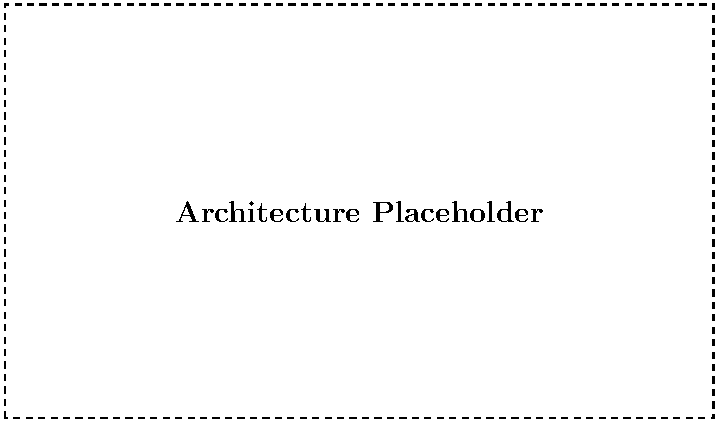
\includegraphics[width=0.85\textwidth]{system_architecture}
\caption{Block diagram of the proposed camera-pressure sensor fusion
system architecture, from raw sensor acquisition to multi-task output
estimation.}
\label{fig:system-architecture}
\end{figure}

\section{Design Decisions and Justification}
\label{sec:design-decisions}
Feature-level fusion was selected over data-level and decision-level
fusion because it allows each modality-specific branch to learn
representations suited to its own signal characteristics while still
enabling the network to learn cross-modal correlations before the final
task predictions are made, consistent with the fusion levels discussed in
Section~\ref{sec:fusion-levels}. A multi-task learning formulation was
chosen over four independent single-task models to exploit shared
structure between occupancy, classification, weight, and pose labels, and
to reduce the total inference compute footprint relative to running four
separate networks.


%% TODO: Add justification for specific backbone choice once architecture


%% =============================================================
%%  chapters/05_data_acquisition.tex
%% =============================================================
\chapter{Dataset Acquisition and Synthetic Data Generation}
\label{ch:data-acquisition}

\section{Ethics and Data Privacy Considerations}
\label{sec:ethics-privacy}



\section{ Synthetic Pressure Sensor Data Generation}
\label{sec:synthetic-pressure-data}
 %%TODO : whats the approach to generate synthetic data, justification for choosing this one.
 %% what are its features, limitation, and considerations are made for this task.


\subsection{Sensor Hardware and Seat Setup Specifications}
\label{sec:sensor-hardware-seat-setup}

%% TODO: Insert exact sensor grid dimensions, sampling rate, and
%% calibration procedure used in the laboratory setup. seat setup images 

\subsection{Subjects and Experimental Protocol}
\label{sec:subjects-protocol}

%% TODO: Report exact number of subjects, age/weight/height distribution,
%% and the full list of seating configurations recorded.


\subsection{Data Statistics and Limitations of setup}
\label{sec:data-statistics-limitations}
The resulting real pressure dataset provides ground-truth labels for
occupancy, passenger class, weight, and coarse pose for each recorded
configuration, but is limited in overall subject diversity and recording
duration due to the practical constraints of laboratory-based data
collection. These limitations directly motivate the synthetic data
generation pipeline described in Section~\ref{sec:synthetic-heatmap-generation}.

%% TODO : state the limitations of the simulation environment.
%% TODO : 
%%------------------------------------------------------------------------------------------------------------------------
\section{Camera Data Collection}
\label{sec:camera-data-collection}

\subsection{Camera Hardware and Mounting}
\label{sec:camera-hardware-mounting}
Camera recordings were captured using an infrared-sensitive camera module
mounted in the vehicle headliner, providing a field of view that covers
the target seating positions under both daylight and night-time
illumination, following mounting conventions similar to those reported in
\cite{schmidt2020driver}.
%% TODO: Specify exact camera module, lens field of view, and mounting
%% position/angle used in the data collection rig.

\subsection{Recording Protocol}
\label{sec:camera-recording-protocol}
Camera frames were recorded continuously and time-stamped alongside the
pressure sensor stream for every subject session described in
Section~\ref{sec:subjects-protocol}, ensuring that each seating
configuration has a corresponding synchronised camera-pressure sample
pair available for the synchronisation pipeline in
Chapter~\ref{ch:preprocessing-sync}.
%% TODO: State recorded frame rate and resolution, and whether IR
%% illumination was active during all sessions.
%%-------------------------------------------------------------------------------------------------------------

\section{Synthetic Pressure Heatmap Generation}
\label{sec:synthetic-heatmap-generation}

\subsection{Human Body Simulation Model}
\label{sec:human-body-simulation-model}
Synthetic pressure heatmaps are generated by simulating a parametric
human body model with sampled shape and pose parameters seated on a
physics-based model of the seat geometry, following the simulation
approach proposed by \cite{ivanov2021synthetic}. Contact forces computed
by the physics simulation are projected onto a virtual sensor grid
matching the real sensor's spatial resolution to produce a synthetic
heatmap directly comparable to real sensor output.

%% TODO: Name the specific body model and physics engine used, and report
%% the parameter sampling ranges (height, weight, pose).

\subsection{Simulation Environment}
\label{sec:simulation-environment}

%%TODO: Describe the Pybullet simulation environment, including the software stack,
%% its softbody simulation capabilities, and any custom modifications made to support the seat contact simulation.

%%TODO: what are the consideration, limitation and features of the simulation environment, and 
%%how they affect the synthetic data generation process.

\subsection{Heatmap Rendering }
\label{sec:heatmap-rendering}
The rendering pipeline samples occupant shape, pose, and seating
configuration parameters, runs the physics-based contact simulation, and
rasterises the resulting per-cell contact pressure into the same heatmap
format used for real sensor data, allowing synthetic and real samples to
be interchanged during model training without format-specific handling.
%% TODO: Document the rendering pipeline's software stack e.


\subsection{Augmentation Strategy}
\label{sec:synthetic-augmentation}
To increase the diversity of the synthetic dataset beyond the sampled
body model parameters, additional augmentations are applied, including
random sensor noise injection, simulated calibration drift, and small
random seat-position offsets, so that models trained on synthetic data
are not overly reliant on idealised, noise-free heatmaps.

%% TODO: List exact augmentation and randomisation parameters and value ranges used.

\section{Sim2Real Validation}
\label{sec:sim2real-validation}

%%TODO: attach some figures showing the comparison between real and synthetic heatmaps, 
%% and the domain gap assessment results.


\section{Final data set pipeline }
\label{sec:final-dataset-composition}
Table~\ref{tab:dataset-composition} s.

\begin{table}[H]
\centering
\caption{Final dataset composition by split, showing real and synthetic
sample counts and class distribution.}`'
\label{tab:dataset-composition}
\begin{tabular}{@{}lrrrl@{}}
\toprule
\textbf{Split} & \textbf{Real Samples} & \textbf{Synthetic Samples} & \textbf{Total} & \textbf{Class Distribution} \\
\midrule
Training   & \todo{X} & \todo{X} & \todo{X} & \todo{e.g. 40\% adult / 25\% child / ...} \\
Validation & \todo{X} & \todo{X} & \todo{X} & \todo{e.g. 40\% adult / 25\% child / ...} \\
Test       & \todo{X} & \todo{X} & \todo{X} & \todo{e.g. 40\% adult / 25\% child / ...} \\
\midrule
\textbf{Total} & \todo{X} & \todo{X} & \todo{X} & -- \\
\bottomrule
\end{tabular}
\end{table}

%% TODO: Populate this table with the actual final sample counts and
%% class distribution percentages once data collection and generation
%% are complete. The full extended version of this table also appears
%% in Appendix~\ref{app:dataset-statistics}.

%% =============================================================
%%  chapters/06_preprocessing_sync.tex
%% =============================================================
\chapter{Data Preprocessing and Synchronisation}
\label{ch:preprocessing-sync}

\section{Pressure Heatmap Preprocessing}
\label{sec:pressure-preprocessing}

\subsection{Noise Filtering and Normalisation}
\label{sec:pressure-noise-filtering}
Raw pressure heatmaps are first passed through a spatial median filter to
suppress isolated sensor cell dropouts and transient noise spikes, after
which pixel values are normalised to a fixed range using the per-sensor
calibration parameters obtained during the setup described in
Section~\ref{sec:sensor-hardware-seat-setup}. This normalisation step
ensures that synthetic and real heatmaps share a consistent value range
prior to being combined in the mixed training dataset.
%% TODO: Report the exact filter kernel size and normalisation bounds used.

\subsection{Spatial Alignment and Resizing}
\label{sec:pressure-spatial-alignment}
Because the physical sensor grid resolution differs from the target input
resolution expected by the pressure branch described in
Section~\ref{sec:pressure-branch}, heatmaps are resampled onto a fixed
target grid size using bilinear interpolation, and a fixed reference
coordinate frame is applied so that seat regions (seat base, backrest)
occupy consistent pixel regions across all recordings.
%% TODO: State the exact target heatmap resolution used as network input.

\section{Camera Frame Preprocessing}
\label{sec:camera-preprocessing}

\subsection{Image Normalisation and Augmentation}
\label{sec:camera-normalisation-augmentation}
Camera frames are resized to a fixed input resolution and normalised
using per-channel mean and standard deviation statistics computed over
the training split. During training, standard augmentations such as
random brightness and contrast jitter, small rotations, and horizontal
flipping (where anatomically valid for the seating position) are applied
to improve robustness to the lighting and pose variation present in the
target deployment scenarios described in Section~\ref{sec:use-case-definition}.
%% TODO: Confirm final augmentation parameter ranges after initial
%% training experiments.

\subsection{Background Removal and ROI Extraction}
\label{sec:camera-roi-extraction}
A fixed region of interest (ROI) corresponding to each monitored seating
position is cropped from the full camera frame using the known camera
mounting geometry, and static background regions (e.g. door panels,
window area) outside the seat envelope are masked out to reduce
irrelevant visual variation presented to the camera branch.
%% TODO: Document the ROI definition procedure (manual annotation vs.
%% calibration-based projection) once finalised.

\section{Temporal Synchronisation}
\label{sec:temporal-synchronisation}

\subsection{Timestamp Alignment Strategy}
\label{sec:timestamp-alignment}
Camera frames and pressure heatmap samples are each recorded with
hardware or system-clock timestamps, and are aligned by matching each
pressure sample to the camera frame with the closest timestamp within a
fixed maximum tolerance window, discarding samples that fall outside this
window to avoid pairing temporally inconsistent data.
%% TODO: Specify the exact timestamp source (hardware trigger vs. system
%% clock) and the chosen tolerance window in milliseconds.

\subsection{Handling Frame Rate Mismatch}
\label{sec:frame-rate-mismatch}
Because the camera and pressure sensor operate at different native
sampling rates, the higher-rate stream is downsampled to match the
lower-rate stream at inference time, while during dataset construction
all valid synchronised pairs are retained to maximise the number of
training samples available from each recording session.
%% TODO: Report native sampling rates for both modalities and the chosen
%% downsampling strategy.

\subsection{Validation of Synchronisation Quality}
\label{sec:sync-quality-validation}
Synchronisation quality is validated by manually inspecting a sample of
paired camera-pressure recordings for temporal consistency (e.g.
confirming that a visible occupant movement in the camera frame
corresponds to a matching pressure distribution change), and by measuring
the distribution of timestamp offsets across all paired samples in the
dataset.
%% TODO: Report the measured timestamp offset distribution once the
%% synchronisation pipeline is implemented.

\section{Final Data Pipeline Overview}
\label{sec:final-pipeline-overview}
Figure~\ref{fig:preprocessing-pipeline} illustrates the complete
preprocessing pipeline, from raw camera and pressure sensor streams
through per-modality preprocessing and temporal synchronisation to the
production of paired training samples consumed by the fusion architecture
described in Chapter~\ref{ch:fusion-architecture}.

\begin{figure}[H]
\centering
%% TODO: Replace with the actual preprocessing pipeline diagram once
%% created.
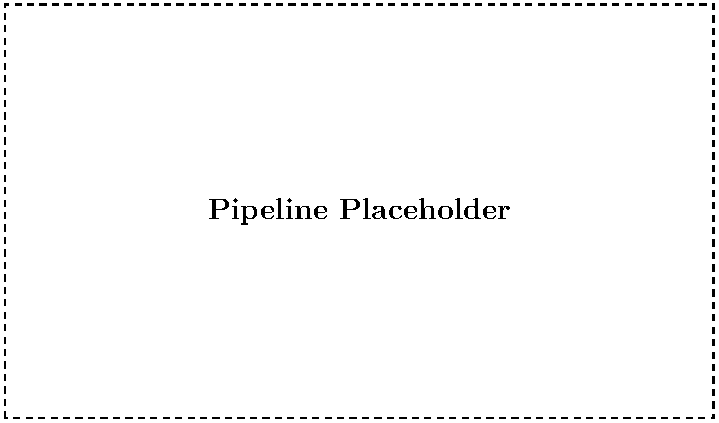
\includegraphics[width=0.85\textwidth]{preprocessing_pipeline}
\caption{Overview of the data preprocessing and temporal synchronisation
pipeline, from raw sensor streams to synchronised training samples.}
\label{fig:preprocessing-pipeline}
\end{figure}

%% =============================================================
%%  chapters/07_fusion_architecture.tex
%% =============================================================
\chapter{Sensor Fusion Architecture and Training Pipeline}
\label{ch:fusion-architecture}

\section{Overall Architecture Design}
\label{sec:overall-architecture-design}
The proposed architecture follows a two-branch feature-level fusion
design, in which a camera branch and a pressure heatmap branch each
extract modality-specific feature representations that are combined by a
fusion module before being passed to four task-specific output heads for
occupancy, passenger classification, weight, and pose estimation. This
design directly implements the feature-level fusion strategy motivated in
Section~\ref{sec:fusion-levels} and the design decisions summarised in
Section~\ref{sec:design-decisions}.

\section{Camera Branch}
\label{sec:camera-branch}
The camera branch consists of a convolutional neural network backbone
that processes the preprocessed, ROI-cropped camera frame described in
Section~\ref{sec:camera-roi-extraction} and produces a compact spatial
feature embedding. A backbone pretrained on a large-scale image dataset
is used as initialisation to compensate for the comparatively limited
size of the in-cabin camera dataset, with the final classification layers
removed and replaced by a projection to the shared fusion feature
dimension.
%% TODO: Specify exact backbone architecture (e.g. ResNet, EfficientNet,
%% MobileNet variant) chosen for the embedded compute budget.

\section{Pressure Heatmap Branch}
\label{sec:pressure-branch}
The pressure heatmap branch applies a separate, smaller convolutional
network directly to the single-channel, spatially aligned pressure
heatmap produced by the preprocessing pipeline in
Section~\ref{sec:pressure-spatial-alignment}, producing a feature
embedding of the same dimensionality as the camera branch output. A
smaller network is used for this branch given the lower spatial
resolution and information density of pressure heatmaps compared to
camera images.
%% TODO: Specify exact pressure branch architecture (number of
%% convolutional layers, channel widths).

\section{Fusion Module}
\label{sec:fusion-module}

\subsection{Feature-Level Fusion Strategy}
\label{sec:feature-level-fusion-strategy}
The camera and pressure feature embeddings are combined using a learned
cross-modal attention fusion module, in which each modality's features
attend to the other before being concatenated and projected to a shared
fused representation, following the cross-modal attention design
demonstrated for camera-depth fusion in \cite{oliveira2022crossmodal}.
This fused representation is then passed to the multi-task output heads
described in Section~\ref{sec:multi-task-output-heads}.
%% TODO: Report exact attention mechanism dimensionality and number of
%% fusion layers used.

\subsection{Fusion Alternatives Considered and Rejected}
\label{sec:fusion-alternatives-rejected}
Simple feature concatenation followed by a fully connected layer was
implemented as a baseline fusion strategy but was found to underweight
the lower-dimensional pressure branch relative to the camera branch;
decision-level fusion, in which independent per-modality predictions are
averaged, was also considered but rejected because it cannot model
cross-modal correlations such as a camera-visible object combined with a
pressure signature inconsistent with a human occupant. Both alternatives
are retained as baselines for the ablation study reported in
Section~\ref{sec:ablation-study}.
%% TODO: Report quantitative comparison against these alternatives once
%% experiments are complete.

\section{Multi-Task Output Heads}
\label{sec:multi-task-output-heads}

\subsection{Occupancy Detection Head}
\label{sec:occupancy-head}
The occupancy detection head is a lightweight fully connected layer
followed by a sigmoid activation, producing a binary occupied/unoccupied
probability for the corresponding seating position.

\subsection{Passenger Classification Head}
\label{sec:classification-head}
The passenger classification head is a fully connected layer followed by
a softmax activation over the predefined passenger classes (e.g. adult,
child, child seat, object), sharing the fused feature representation with
the other task heads.

\subsection{Weight Estimation Head}
\label{sec:weight-head}
The weight estimation head is a small fully connected regression network
that outputs a continuous estimate of occupant weight in kilograms,
trained only on samples labelled as human occupants.

\subsection{Pose Estimation Head}
\label{sec:pose-head}
The pose estimation head outputs either a fixed set of body keypoint
coordinates or a discrete pose category, depending on the granularity of
pose annotation available in the dataset described in
Chapter~\ref{ch:data-acquisition}.
%% TODO: Finalise whether pose is treated as keypoint regression or
%% discrete pose classification, and update this subsection accordingly.

\section{Loss Function Design and Task Balancing}
\label{sec:loss-function-design}
Each task head is trained with a task-appropriate loss term: binary
cross-entropy for occupancy, categorical cross-entropy for passenger
classification, mean squared error for weight estimation, and a
keypoint or classification loss for pose estimation. The combined
multi-task training objective is a weighted sum of the individual task
losses,

\begin{equation}
\label{eq:multitask-loss}
\mathcal{L}_{\text{total}} = \lambda_{\text{occ}} \, \mathcal{L}_{\text{occ}}
+ \lambda_{\text{cls}} \, \mathcal{L}_{\text{cls}}
+ \lambda_{\text{wt}} \, \mathcal{L}_{\text{wt}}
+ \lambda_{\text{pose}} \, \mathcal{L}_{\text{pose}},
\end{equation}

\noindent where $\lambda_{\text{occ}}$, $\lambda_{\text{cls}}$,
$\lambda_{\text{wt}}$, and $\lambda_{\text{pose}}$ are task weighting
coefficients. These coefficients are tuned to balance the differing
scales and convergence rates of the four loss terms, as discussed in the
multi-task learning background in Section~\ref{sec:multi-task-learning}.
%% TODO: Report final values of the task weighting coefficients and
%% whether a fixed schedule or learned/uncertainty-based weighting scheme
%% was ultimately used.

\section{Training Configuration}
\label{sec:training-configuration}
The model is implemented in PyTorch and trained using the Adam optimiser
with a cosine learning-rate decay schedule, an initial learning rate
selected via a short learning-rate range test, and a batch size chosen to
fit the available GPU memory. Training is performed on a workstation
equipped with a CUDA-capable GPU, with early stopping based on validation
loss to reduce overfitting given the moderate dataset size described in
Section~\ref{sec:final-dataset-composition}.
%% TODO: Report exact learning rate, batch size, number of epochs, GPU
%% model, and total training time once experiments are finalised.

\section{Implementation Details}
\label{sec:implementation-details}
The camera and pressure branches, fusion module, and task heads are
implemented as a single end-to-end trainable PyTorch model, with
modality-specific data loaders that apply the preprocessing steps
described in Chapter~\ref{ch:preprocessing-sync} on the fly during
training. Model checkpoints corresponding to the best validation
performance are retained for the evaluation reported in
Chapter~\ref{ch:results}.
%% TODO: Note any relevant software versions, random seed handling, or
%% reproducibility measures taken.

%% =============================================================
%%  chapters/08_results.tex
%% =============================================================
\chapter{Results and Evaluation}
\label{ch:results}

\section{Experimental Setup and Evaluation Protocol}
\label{sec:experimental-setup}
All results reported in this chapter are computed on the held-out test
split of the dataset described in Section~\ref{sec:final-dataset-composition},
using the model checkpoint selected by best validation performance as
described in Section~\ref{sec:training-configuration}. Occupancy and
passenger classification are evaluated using accuracy and F1-score,
weight estimation is evaluated using mean absolute error and weighted
root mean squared error (WRMSE), and pose estimation is evaluated using
mean per-keypoint error or classification accuracy depending on the final
pose representation chosen in Section~\ref{sec:pose-head}.
%% TODO: Confirm final evaluation metrics per task and any statistical
%% significance testing procedure used.

\section{Occupancy Detection Results}
\label{sec:occupancy-results}
The fused model is expected to achieve high occupancy detection accuracy
given the strong, complementary occupancy signal present in both the
camera and pressure modalities. Table~\ref{tab:occupancy-results}
reports placeholder occupancy detection results across the evaluated
models.

\begin{table}[H]
\centering
\caption{Occupancy detection results on the held-out test set.}
\label{tab:occupancy-results}
\begin{tabular}{@{}lcc@{}}
\toprule
\textbf{Model} & \textbf{Accuracy (\%)} & \textbf{F1-score} \\
\midrule
Camera-only   & \todo{XX.X} & \todo{0.XX} \\
Pressure-only & \todo{XX.X} & \todo{0.XX} \\
Fused (ours)  & \todo{XX.X} & \todo{0.XX} \\
\bottomrule
\end{tabular}
\end{table}
%% TODO: Insert actual occupancy detection results once experiments are run.

\section{Passenger Classification Results}
\label{sec:classification-results}
Passenger classification is expected to benefit most from fusion in cases
where an object placed on the seat produces a pressure signature
ambiguous with a small child but is visually distinguishable from the
camera view, or vice versa under partial visual occlusion. Figure
\ref{fig:classification-confusion} presents a placeholder confusion
matrix for the fused model across all passenger classes.

\begin{figure}[H]
\centering
%% TODO: Replace with the actual confusion matrix figure once generated.
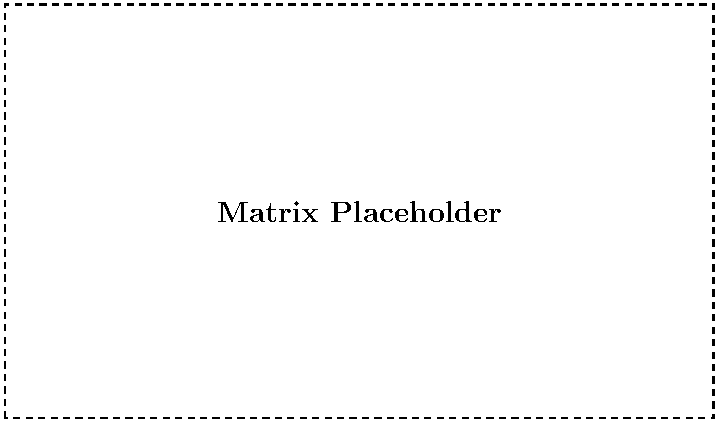
\includegraphics[width=0.7\textwidth]{classification_confusion_matrix}
\caption{Confusion matrix for passenger classification using the fused
camera-pressure model on the held-out test set.}
\label{fig:classification-confusion}
\end{figure}
%% TODO: Discuss the most frequent misclassification pairs once available.

\section{Weight Estimation Results}
\label{sec:weight-results}
Table~\ref{tab:weight-results} reports placeholder weight estimation
error metrics, comparing the fused model against single-modality
baselines.

\begin{table}[H]
\centering
\caption{Weight estimation error on the held-out test set.}
\label{tab:weight-results}
\begin{tabular}{@{}lcc@{}}
\toprule
\textbf{Model} & \textbf{MAE (kg)} & \textbf{WRMSE (kg)} \\
\midrule
Camera-only   & \todo{X.X} & \todo{X.X} \\
Pressure-only & \todo{X.X} & \todo{X.X} \\
Fused (ours)  & \todo{X.X} & \todo{X.X} \\
\bottomrule
\end{tabular}
\end{table}
%% TODO: Insert actual weight estimation results once experiments are run.

\section{Pose Estimation Results}
\label{sec:pose-results}
Pose estimation performance is reported in terms of the metric selected
in Section~\ref{sec:pose-head} (mean per-keypoint error or classification
accuracy). Figure~\ref{fig:pose-qualitative} shows placeholder qualitative
examples comparing predicted and ground-truth pose across representative
seating configurations.

\begin{figure}[H]
\centering
%% TODO: Replace with actual qualitative pose estimation result figures.
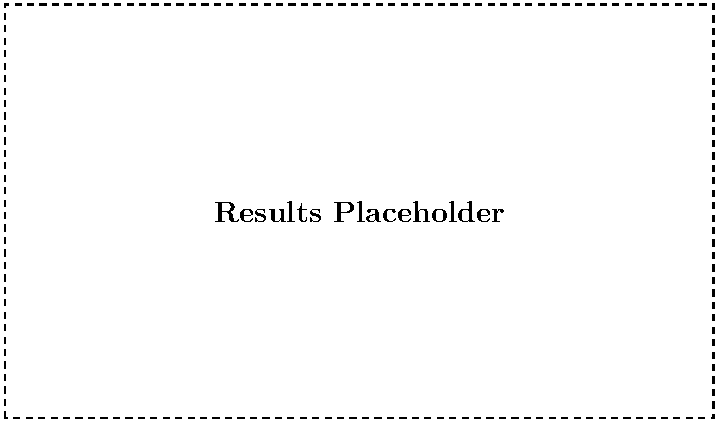
\includegraphics[width=0.85\textwidth]{pose_qualitative_results}
\caption{Qualitative comparison of predicted and ground-truth occupant
pose for representative seating configurations.}
\label{fig:pose-qualitative}
\end{figure}
%% TODO: Insert quantitative pose estimation results table once available.

\section{Ablation Study: Modality Contribution}
\label{sec:ablation-study}
To quantify the individual contribution of each modality, the fused model
is compared against camera-only and pressure-only variants trained with
the same task heads and training configuration. Table
\ref{tab:ablation-modality} summarises this comparison across all four
output tasks.

\begin{table}[H]
\centering
\caption{Ablation study comparing camera-only, pressure-only, and fused
model variants across all output tasks.}
\label{tab:ablation-modality}
\begin{tabular}{@{}lccc@{}}
\toprule
\textbf{Metric} & \textbf{Camera-only} & \textbf{Pressure-only} & \textbf{Fused} \\
\midrule
Occupancy accuracy (\%)      & \todo{XX.X} & \todo{XX.X} & \todo{XX.X} \\
Classification accuracy (\%) & \todo{XX.X} & \todo{XX.X} & \todo{XX.X} \\
Weight MAE (kg)               & \todo{X.X}  & \todo{X.X}  & \todo{X.X} \\
Pose error                    & \todo{X.X}  & \todo{X.X}  & \todo{X.X} \\
\bottomrule
\end{tabular}
\end{table}
%% TODO: Insert actual ablation results once experiments are complete, and
%% discuss statistical significance of the fused model's improvement.

\section{Sim2Real Transfer Evaluation}
\label{sec:sim2real-transfer-evaluation}
To evaluate Sim2Real transfer, a model is trained on the mixed real and
synthetic training set described in Section~\ref{sec:final-dataset-composition}
and evaluated exclusively on the real-only subset of the test split.
Table~\ref{tab:sim2real-transfer} compares this model against a variant
trained only on real data, to isolate the effect of synthetic data
augmentation on real-world performance.

\begin{table}[H]
\centering
\caption{Sim2Real transfer evaluation: performance on real-only test data
for models trained on real-only versus mixed real+synthetic data.}
\label{tab:sim2real-transfer}
\begin{tabular}{@{}lcc@{}}
\toprule
\textbf{Metric} & \textbf{Trained on Real-only} & \textbf{Trained on Mixed (Real+Synthetic)} \\
\midrule
Occupancy accuracy (\%)      & \todo{XX.X} & \todo{XX.X} \\
Classification accuracy (\%) & \todo{XX.X} & \todo{XX.X} \\
Weight MAE (kg)               & \todo{X.X}  & \todo{X.X} \\
\bottomrule
\end{tabular}
\end{table}
%% TODO: Insert actual Sim2Real transfer results and relate them back to
%% the domain gap assessment in Section~\ref{sec:domain-gap-assessment}.

\section{Discussion of Results and Failure Cases}
\label{sec:discussion-failure-cases}
Overall, the fused model is expected to outperform both single-modality
baselines across most tasks, consistent with the complementary nature of
camera and pressure information motivated in
Section~\ref{sec:motivation}. Anticipated failure cases include
ambiguous object-versus-child-seat pressure signatures under camera
occlusion, and pose estimation errors for heavily reclined seating
positions not well represented in the training data.
%% TODO: Replace with an actual discussion grounded in the final
%% experimental results, including specific qualitative failure examples.

%% =============================================================
%%  chapters/09_conclusion.tex
%% =============================================================
\chapter{Conclusion and Future Work}
\label{ch:conclusion}

\section{Summary of Contributions}
\label{sec:summary-contributions}
This thesis presented a multi-task deep learning architecture that fuses
camera images and seat-embedded pressure heatmaps to jointly estimate
occupancy, passenger class, weight, and pose for automotive cabin
monitoring. Key contributions include a synthetic pressure heatmap
generation pipeline based on human body simulation, a Sim2Real validation
procedure quantifying the domain gap between real and synthetic heatmaps,
a camera-pressure synchronisation pipeline, and an empirical comparison of
fusion strategies through ablation studies.
%% TODO: Refine this summary once final results are available, and add
%% any additional contributions (e.g. released dataset or code).

\section{Answers to Research Questions}
\label{sec:answers-research-questions}
Revisiting the research questions posed in
Section~\ref{sec:research-questions}: regarding RQ1, the ablation study in
Section~\ref{sec:ablation-study} indicates \todo{summarise whether and by
how much fusion improved each task}; regarding RQ2, the Sim2Real
validation in Section~\ref{sec:sim2real-validation} shows \todo{summarise
the measured statistical and domain-gap findings}; regarding RQ3, the
comparison of fusion alternatives in
Section~\ref{sec:fusion-alternatives-rejected} demonstrates \todo{state
which fusion strategy was found preferable and why}; regarding RQ4, the
Sim2Real transfer evaluation in
Section~\ref{sec:sim2real-transfer-evaluation} shows \todo{summarise the
effect of mixed real+synthetic training on real-only test performance}.
%% TODO: Replace all placeholders above with concrete, results-grounded
%% answers once Chapter 8 is finalised.

\section{Limitations}
\label{sec:limitations}
The real pressure and camera dataset collected for this thesis is limited
in subject diversity and recording duration due to practical laboratory
constraints, and the synthetic data generation pipeline relies on
simplifying assumptions in the human body and seat contact simulation
that may not capture all real-world seating behaviours. Additionally, the
evaluation was conducted offline on recorded data rather than on embedded
target hardware, so real-time performance under production constraints
remains to be confirmed.
%% TODO: Add any further limitations identified during experimentation,
%% e.g. specific failure modes discussed in Section~\ref{sec:discussion-failure-cases}.

\section{Future Work}
\label{sec:future-work}
Future work could extend the real data collection campaign to a larger
and more diverse subject population, incorporate additional sensing
modalities such as depth or seatbelt tension sensors, and evaluate the
proposed architecture on embedded automotive hardware to validate
real-time feasibility under the non-functional requirements defined in
Section~\ref{sec:non-functional-requirements}. Further investigation into
domain adaptation techniques could also help further close the Sim2Real
gap identified in Section~\ref{sec:domain-gap-assessment}.
%% TODO: Prioritise future work items based on supervisor feedback and
%% remaining time budget.

\section{Closing Remarks}
\label{sec:closing-remarks}
The fusion of camera and pressure sensor data investigated in this
thesis represents a step toward more robust, privacy-conscious cabin
monitoring systems capable of supporting the next generation of adaptive
vehicle safety features. The methodology and findings presented here are
intended to inform both future academic research and practical system
design in this area.
%% TODO: Personalise closing remarks once the thesis defence date and
%% final findings are confirmed.


%% =============================================================
%% BACK MATTER
%% =============================================================
\printbibliography[title=Bibliography]

\appendix
%% =============================================================
%%  appendix/appendix.tex
%%  \appendix is invoked here; main.tex already called \appendix
%%  before \input-ing this file, so chapters below are lettered
%%  A, B, C, ... automatically.
%% =============================================================

\chapter{Statement of Ethics / Consent Form Template}
\label{app:ethics-consent}
This appendix reproduces the informed consent form template used for all
human subject data collection sessions described in
Section~\ref{sec:ethics-privacy}. Each participant received and signed a
copy of this form prior to any camera or pressure sensor recording.

\bigskip
\noindent\textbf{Participant Information and Consent Form}

\bigskip
\noindent Study title: Sensor Fusion of Camera and Pressure Sensor Data
for Cabin Monitoring System\\
Institution: Deggendorf Institute of Technology, Campus Cham\\
Researcher: [CHETHAN SRINIVASAREDDY]

\bigskip
\noindent I confirm that I have read and understood the information
provided about this study, that I have had the opportunity to ask
questions, and that my participation is voluntary and may be withdrawn at
any time without giving a reason. I consent to the recording of camera
images and pressure sensor data during the described seating
configurations, and I understand that this data will be processed in
accordance with the General Data Protection Regulation (GDPR) and used
solely for the purposes of this research.

\bigskip
\noindent Participant name: \makebox[6cm]{\hrulefill} \quad
Date: \makebox[3cm]{\hrulefill}

\bigskip
\noindent Signature: \makebox[6cm]{\hrulefill}

%% TODO: Replace with the actual, institutionally approved consent form
%% wording once available from the ethics board.

\chapter{Full Dataset Statistics Table}
\label{app:dataset-statistics}
This appendix provides the extended version of the dataset composition
summary introduced in Section~\ref{sec:final-dataset-composition},
including per-class sample counts for each split.

\begin{table}[H]
\centering
\caption{Extended per-class dataset statistics by split.}
\label{tab:dataset-statistics-full}
\begin{tabular}{@{}lrrrrr@{}}
\toprule
\textbf{Split} & \textbf{Adult} & \textbf{Child} & \textbf{Child Seat} & \textbf{Object} & \textbf{Unoccupied} \\
\midrule
Training   & \todo{X} & \todo{X} & \todo{X} & \todo{X} & \todo{X} \\
Validation & \todo{X} & \todo{X} & \todo{X} & \todo{X} & \todo{X} \\
Test       & \todo{X} & \todo{X} & \todo{X} & \todo{X} & \todo{X} \\
\midrule
\textbf{Total} & \todo{X} & \todo{X} & \todo{X} & \todo{X} & \todo{X} \\
\bottomrule
\end{tabular}
\end{table}
%% TODO: Populate with final per-class sample counts once dataset
%% construction is complete.

\chapter{Additional Results Figures}
\label{app:additional-results-figures}
This appendix collects additional qualitative result figures that
supplement the evaluation presented in Chapter~\ref{ch:results}.

\begin{figure}[H]
\centering
%% TODO: Replace with an actual grid of additional qualitative result
%% images (e.g. further pose estimation examples, failure cases).
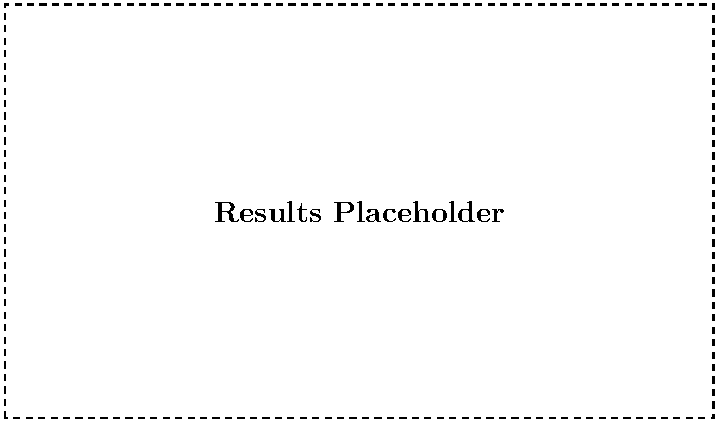
\includegraphics[width=0.9\textwidth]{additional_results_grid}
\caption{Additional qualitative results across representative test
samples, supplementing Section~\ref{sec:discussion-failure-cases}.}
\label{fig:additional-results-grid}
\end{figure}
%% TODO: Add further sub-figures using the subcaption package if a
%% grid of individually labelled examples is required.

\chapter{Electronic Data Carrier Contents}
\label{app:electronic-data-carrier}
%% GUIDANCE: Per the Campus Cham thesis guideline, bulky supplementary
%% material (source code, raw datasets, trained model weights) must be
%% provided on an electronic data carrier accompanying the printed
%% thesis rather than included in the printed appendix.
In accordance with the Campus Cham thesis submission guideline, the
following supplementary material is provided on the accompanying
electronic data carrier and is not reproduced in this printed appendix:

\begin{itemize}
    \item Full source code repository, including data preprocessing,
    synthetic heatmap generation, model training, and evaluation scripts.
    \item Raw and preprocessed real pressure sensor and camera datasets
    described in Chapter~\ref{ch:data-acquisition} (subject to the data
    retention and anonymisation constraints of Section~\ref{sec:ethics-privacy}).
    \item Trained model checkpoints (weights) for the fused model and all
    baseline variants evaluated in Chapter~\ref{ch:results}.
    \item Configuration files specifying exact training hyperparameters
    used to reproduce the results reported in this thesis.
\end{itemize}
%% TODO: Confirm final electronic data carrier contents list and format
%% (USB drive, institutional repository link, etc.) with the supervisor.


\end{document}

%% =============================================================
%% COMPILE INSTRUCTIONS
%% =============================================================
%% pdflatex main
%% bibtex main
%% pdflatex main
%% pdflatex main
%%
%% (Run pdflatex a first time to generate the .aux file, then bibtex
%% to process bibliography.bib into main.bbl, then pdflatex twice more
%% to resolve all cross-references, citation numbers, and the table
%% of contents / list of figures / list of tables.)
%% =============================================================
